\DocumentMetadata{
	lang		= eng-US,
	pdfstandard	= A-3u,
	pdfversion	= 1.7,
}

\documentclass[colorlinks,upint,balance]{asmeconf}

\usepackage{graphicx}
\usepackage{booktabs}
\usepackage{multirow}

\hypersetup{%
	pdfauthor={J.C. Vaught},
	pdftitle={Effect of Echo Trail Parameters on YOLO-Based Target Detection in Simulated Marine Radar Imagery},
	pdfkeywords={echo trails, marine radar, YOLO, object detection, PPI, radar simulation},
}

\begin{document}

\ConfName{Proceedings of the ASME 2026\linebreak International Design Engineering Technical Conferences \&\linebreak Computers and Information in Engineering Conference}
\ConfAcronym{IDETC/CIE 2026}
\ConfDate{August 23--26, 2026}
\ConfCity{Houston, TX}
\PaperNo{IDETC2026-XXXXX}

\title{Effect of Echo Trail Parameters on YOLO-Based Target Detection in Simulated Marine Radar Imagery}

\SetAuthors{%
	J.C. Vaught\affil{1}\CorrespondingAuthor{jvaught@sc.edu},
	Douglas Cahl\affil{1},
	Yi Wang\affil{1}
}

\SetAffiliation{1}{Department of Mechanical Engineering, University of South Carolina, Columbia, SC}

\maketitle

\begin{figure*}[t]
\centering
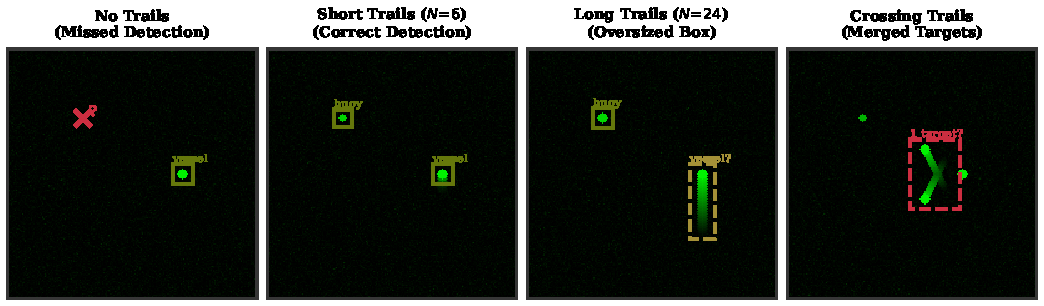
\includegraphics[width=\textwidth]{figures/fig0_splash.pdf}
\caption{The echo trail problem for machine learning detectors. The same radar scene rendered with different trail configurations produces dramatically different detection outcomes. Without trails, a faint buoy is missed entirely. With well-tuned short trails, both buoy and vessel are correctly detected. With excessively long trails, the vessel's bounding box becomes oversized due to streak artifacts. When two targets on crossing tracks produce overlapping trails, the detector merges them into a single detection. \textit{Placeholder---replace with real radar imagery and YOLO inference results.}}
\label{fig:splash}
\end{figure*}

\begin{figure}[t]
\centering
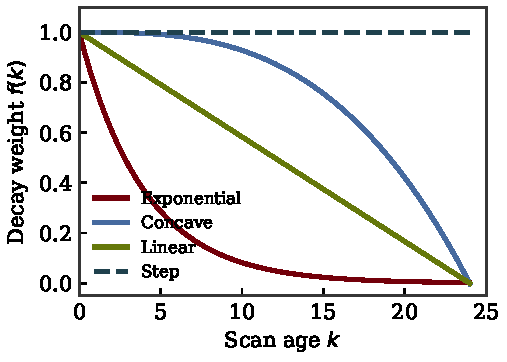
\includegraphics[width=\columnwidth]{figures/fig1_decay_functions.pdf}
\caption{The four decay functions investigated in this study. Exponential decay fades quickly with a long tail. Concave decay ($p=3$) holds intensity before dropping sharply. Linear decay fades uniformly. Step decay maintains full intensity until a hard cutoff. \textit{Placeholder---replace with actual implementation output.}}
\label{fig:decay_functions}
\end{figure}

\keywords{echo trails, marine radar, YOLO, object detection, PPI, radar simulation, deep learning}

% ====================================================================
% ABSTRACT
% ====================================================================
\begin{abstract}
Echo trails---the persistence of radar returns across successive PPI scans---appear on every marine radar display, yet their effect on deep learning detectors has never been studied. This paper presents a systematic ablation study of how trail length, decay function, intensity encoding, color mapping, target range, clutter level, target proximity, and trajectory crossing influence YOLOv8 detection performance on simulated X-Band marine radar imagery. Results reveal that trail parameters substantially affect detection accuracy, that optimal trail length depends on both target range and speed, and that crossing trajectories produce overlap artifacts that degrade multi-target resolution. These findings motivate range-adaptive trail rendering as a design principle for machine-learning-driven maritime perception.
\end{abstract}


% ====================================================================
% 1  INTRODUCTION
% ====================================================================
\section{Introduction}

For over half a century, marine radar has served as the primary sensor for navigational safety in occluded waterways, adverse weather, and military operations~\cite{Skolnik2001Radar}. Despite this ubiquity, reliably detecting, classifying, and tracking targets in radar imagery remains an open problem. Small targets vanish in sea clutter, closely spaced objects merge into single returns, and moving targets produce spatial artifacts that confuse both human operators and automated systems~\cite{Ward2013Marine, Chen2022VisibilityGraph}. The research community has attacked this problem from two directions---signal processing at the receiver and deep learning on the display---with significant progress but persistent limitations.

On the signal processing side, the community has pursued progressively more sophisticated approaches to extract targets from noise. In 1983, Rohling~\cite{Rohling1983CFAR} introduced CFAR processing, adapting detection thresholds to local clutter statistics. The primary limitation of CFAR---the lack of temporal information---was addressed in 2012 when Kim et al.~\cite{Kim2012ScanCorrelation} correlated returns across consecutive antenna sweeps to improve weak target detection. In doing so, however, they discovered that temporal accumulation introduces ``target tail'' artifacts that degrade detection of fast-moving objects, and proposed signal-level suppression to eliminate them. Wen et al.~\cite{Wen2022SpatioTemporal} pushed further in 2022, applying 3D-FFT filtering across radar image sequences to achieve 15.3~dB of signal-to-noise improvement. Despite these advances, each method operates upstream of the display---improving what the radar captures, never examining what the detector ultimately sees.

On the deep learning side, neural networks have moved from processing raw radar signals to treating the rendered PPI display as a standard object detection problem. Early work by Vicen-Bueno et al.~\cite{VicenBueno2009Neural} in 2009 applied neural networks to sea clutter reduction at the signal level. By 2020, Baird et al.~\cite{Baird2020CNNLSTM} had shifted to CNN-LSTM architectures operating directly on display imagery, and in 2021 Chen et al.~\cite{Chen2021PPInet} achieved 15\% detection improvement over CA-CFAR using YOLOv3 on PPI images. Increasingly powerful architectures followed through 2025~\cite{Wang2023SALALSTM, Yin2023SWFormer, Jia2025YOLOv11OBB}. The most revealing development, however, came from systems that explicitly incorporate temporal information across consecutive scans---Chen et al.'s multi-frame fusion in PPInet and DTNet's~\cite{DTNet2025MultiFrame} multi-frame PPI inputs, which achieved 99\% precision. These systems accumulate returns across successive antenna sweeps to improve detection---yet they do so on display images where temporal accumulation has already been applied by the rendering layer. Despite explicitly exploiting the same phenomenon, not one of these systems examined how the existing accumulation in their input shaped the features they sought to learn.

Those display images contain echo trails---configurable persistence from previous antenna scans~\cite{Briggs2004RadarDisplay}. The International Maritime Organization mandated them on all shipborne radar in 2004~\cite{IMO2004MSC192}, and the International Electrotechnical Commission codified test procedures in IEC~62388~\cite{IEC2013Radar}---yet neither body specifies which configuration is optimal, because no empirical study has ever informed that question. The ``target tails'' that Kim et al. sought to suppress at the signal level are the same phenomenon, rendered deliberately on every radar display not as a defect but as a feature. Despite decades of deployment, regulatory mandate, and an expanding body of ML research built on trailed imagery, no one has examined how trail configuration affects detection. Figure~\ref{fig:splash} illustrates what is at stake: the same scene rendered with different configurations produces dramatically different detection outcomes.

The problem cannot be resolved by intuition. A target moving at 10~knots produces large pixel displacement per scan at near range and negligible displacement at far range---meaning the same trail length that improves detection at one range may degrade it at another~\cite{Chen2022VisibilityGraph}. This range dependence interacts with decay shape, intensity encoding, and color mapping in ways that cannot be predicted without controlled experimentation. Isolating these interactions requires holding all other variables constant, which is infeasible on operational radar---motivating the use of simulation, where Ting and Greenspan~\cite{Ting2023SyntheticRadar} demonstrated in 2023 that synthetic radar data can effectively substitute for real hardware in parametric studies of this kind.

This paper presents the first systematic investigation of how echo trail parameters affect deep learning detection on marine radar imagery (Fig.~\ref{fig:pipeline}). We employ an RCS-based radar simulator that generates PPI imagery matching the output format of real marine radar hardware, then implement configurable echo trail rendering as a post-processing layer. Through eight sequential ablation experiments---each isolating one parameter while holding the rest at the best previously identified configuration---we map the relationship between trail length, decay shape, intensity encoding, color mapping, and YOLOv8 detection performance. The contributions are fourfold. First, we quantify the sensitivity of detection performance to each trail parameter across multiple target speed classes (Sec.~5.1--5.4). Second, we demonstrate that optimal trail length depends on target range, motivating range-adaptive trail rendering (Sec.~5.5). Third, we characterize the degradation caused by trail overlap when targets on crossing trajectories produce intersecting streaks (Sec.~5.8). Fourth, we provide practical recommendations for configuring echo trail rendering in machine-learning-driven radar perception pipelines (Sec.~7).


% ====================================================================
% 2  BACKGROUND
% ====================================================================
\section{Background}

\subsection{Echo Trails on Marine Radar}

Echo trails, also referred to as target trails or radar persistence, are a display-side feature that retains returns from previous antenna scans and renders them with progressively reduced intensity~\cite{Briggs2004RadarDisplay}. On a conventional PPI display, each pixel's intensity reflects not only the current scan's return at that range-bearing cell but also a weighted combination of returns from $N$ previous scans. The trail length $N$ determines how many past scans contribute, while the decay function $f(k)$ specifies the weight assigned to the return from $k$ scans ago.

This study investigates four decay functions that span the space of practically relevant temporal profiles (Fig.~\ref{fig:decay_functions}). \textit{Exponential} decay produces rapid initial fading followed by a long tail of low-intensity persistence, governed by a time constant $\tau$.
\begin{align}
	f_{\mathrm{exp}}(k) = e^{-k/\tau}, \quad k = 0, 1, \ldots, N
	\label{eq:exp_decay}
\end{align}
\textit{Concave} decay maintains near-full intensity for most of the trail history, then drops sharply near the end, parameterized by an exponent $p > 1$.
\begin{align}
	f_{\mathrm{conc}}(k) = \max\!\left(0,\; 1 - \left(\frac{k}{N}\right)^{p}\right), \quad k = 0, 1, \ldots, N
	\label{eq:concave_decay}
\end{align}
\textit{Linear} decay assigns weights that decrease uniformly with scan age.
\begin{align}
	f_{\mathrm{lin}}(k) = 1 - \frac{k}{N}, \quad k = 0, 1, \ldots, N
	\label{eq:linear_decay}
\end{align}
\textit{Step} (fixed) decay retains full intensity for all $N$ scans, then drops to zero.
\begin{align}
	f_{\mathrm{step}}(k) = \begin{cases} 1, & k \leq N \\ 0, & k > N \end{cases}
	\label{eq:step_decay}
\end{align}

These four functions span a spectrum from rapid-fade-with-persistence (exponential) through uniform fade (linear) to full-retention-with-hard-cutoff (step), with concave decay occupying the intermediate regime of slow initial fade and rapid terminal drop. On PPI imagery, these profiles produce visually distinct trail signatures: exponential decay yields a rapidly fading tail, concave decay retains near-full intensity before dropping sharply, linear decay fades uniformly, and step decay creates a uniform-intensity streak with an abrupt cutoff.

\subsection{YOLO Object Detection}

The YOLO architecture~\cite{Redmon2016YOLO} reframed object detection as a single regression problem, predicting bounding boxes and class probabilities in one forward pass. YOLOv8~\cite{Jocher2023YOLOv8} introduced an anchor-free detection head, while YOLOv9~\cite{Wang2024YOLOv9} incorporated programmable gradient information to reduce information loss. For radar PPI imagery, YOLO's single-stage design is attractive because PPI images contain few object classes, targets tend to be small, and real-time inference is essential.

\subsection{Temporal Information in Detection}

Feichtenhofer et al.~\cite{Feichtenhofer2017Temporal} demonstrated that jointly performing detection and tracking in video improves both tasks. Zhu et al.~\cite{Zhu2017FlowGuided} showed that deep feature flow can accelerate video recognition without sacrificing accuracy. Echo trails encode temporal information directly into a single image, providing implicit temporal context that a single-frame detector can exploit without multi-frame processing. Whether this implicit encoding helps or hurts detection---and under what trail configurations---is the central question of this study.


% ====================================================================
% 3  SIMULATION FRAMEWORK
% ====================================================================
\section{Simulation Framework}

\begin{figure*}[t]
\centering

\includegraphics[width=\textwidth]{figures/fig_pipeline.pdf}
\caption{Processing pipeline for the echo trail ablation study. The RCS simulator generates raw PPI frames from scene descriptions. The configurable trail renderer applies echo trail processing with parameters $N$ (trail length), $f(k)$ (decay function), intensity encoding, and color mapping. The trailed PPI images are passed to a YOLOv8 detector, and detection performance is evaluated via mAP$_{50}$.}
\label{fig:pipeline}
\end{figure*}

\subsection{RCS-Based Radar Simulator}

The radar simulator generates synthetic PPI imagery based on radar cross section (RCS) modeling of scene objects. The simulator accepts a scene description consisting of target positions, RCS profiles, and motion trajectories, then computes received power at each range-bearing cell according to the radar range equation~\cite{Richards2014Fundamentals}. Sea clutter is modeled using K-distributed random variates~\cite{Ward2013Marine}, and thermal noise is added as additive white Gaussian noise. The output is a sequence of PPI images at the antenna rotation rate, quantized to match the bit depth and format of real radar hardware (4-bit intensity, polar-to-Cartesian mapped). The simulator's output format is identical to that produced by the Furuno DRS4D-NXT radar sensor~\cite{Furuno2020DRS4DNXT}, enabling direct comparison with real hardware imagery.

\subsection{Echo Trail Implementation}

Echo trails are implemented as a configurable post-processing layer. For each pixel at position $(r, \theta)$ on the PPI at scan $t$, the displayed intensity is computed as the maximum of the weighted history.
\begin{align}
	I_{\mathrm{disp}}(r, \theta, t) = \max_{k=0}^{N} \left[ f(k) \cdot I_{\mathrm{raw}}(r, \theta, t-k) \right]
	\label{eq:trail_composite}
\end{align}
The $\max$ operator ensures that a strong current return is never attenuated by weaker historical returns, consistent with standard radar display behavior. The physical consequence of this compositing depends strongly on range: the same physical target speed produces dramatically different pixel displacement at different ranges, resulting in trail footprints that vary from compact reinforcement at far range to elongated streaks at near range. Trail-induced streaks also affect detection evaluation, because increasing trail length progressively degrades the intersection-over-union (IoU) between predicted and ground truth bounding boxes---a mechanism quantified in Section~5.

\subsection{Trail Intensity Encoding}

A key design choice is how the original return strength maps into trail pixel intensity. In \textit{binary} encoding, any non-zero return produces a trail pixel at full intensity---a navigation buoy with a faint return and a steel-hulled vessel with a strong return produce identical trail pixels. In \textit{proportional} encoding, the trail pixel intensity scales with the original return strength, preserving radiometric information in the trail. Binary encoding is simpler and produces higher-contrast trails, but discards information that the detector could potentially exploit to distinguish target types.

\subsection{Color Mapping}

Color mapping transforms the scalar trail intensity to an RGB pixel value. Four strategies are investigated. \textit{Monochrome} applies a single-channel intensity scale (green-on-black). \textit{Two-tone} renders current returns in one color and all trail pixels in a contrasting color. \textit{Gradient} maps trail age to a continuous color ramp (e.g., green $\rightarrow$ yellow $\rightarrow$ red). \textit{Intensity-mapped} assigns color based on the original return strength rather than trail age, encoding target type information in the hue channel.


% ====================================================================
% 4  EXPERIMENTAL DESIGN
% ====================================================================
\section{Experimental Design}

\subsection{Ablation Structure}

The study is structured as eight sequential ablation experiments (Table~\ref{tab:ablations}). Each ablation varies one parameter while holding all others at the best configuration identified in prior ablations, avoiding a full factorial design. A1 sweeps trail length across four speed classes (stationary, 2, 5, and 15~px/scan). A2 compares decay functions at the best $N$ from A1. A3 evaluates binary versus proportional intensity encoding on mixed-strength scenes. A4 tests four color schemes. A5 re-sweeps trail length at near ($\sim$200~m), mid ($\sim$1~nm), and far ($\sim$3~nm) ranges. A6 evaluates clutter interaction. A7 measures the merging threshold for closely spaced stationary targets. A8 evaluates crossing-trajectory trail overlap at varying angles. The no-trail condition ($N=0$) is the universal baseline. All models are trained on YOLOv8~\cite{Jocher2023YOLOv8} from a common pretrained checkpoint, with 400 training frames and 100 test frames per condition.

\begin{table}[t]
\caption{Ablation experiments.}
\label{tab:ablations}
\centering
\footnotesize
\begin{tabular}{@{}lll@{}}
\toprule
 & \textbf{Variable} & \textbf{Levels} \\
\midrule
A1 & Trail length & $N \in \{0,3,6,12,24\}$ \\
A2 & Decay function & Exp, Conc, Lin, Step \\
A3 & Intensity mode & Binary, Proportional \\
A4 & Color mapping & Mono, 2-tone, Grad, Int. \\
A5 & Target range & Near, Mid, Far \\
A6 & Clutter level & Low, Moderate, Heavy \\
A7 & Proximity & 10--100\,m separation \\
A8 & Crossing tracks & $15^\circ$--$90^\circ$ angle \\
\bottomrule
\end{tabular}
\end{table}

\subsection{Target Speed Parameterization}

Target speed is parameterized as apparent pixel displacement per scan rather than physical velocity. This captures the joint effect of physical speed, range, and antenna rotation rate on the trail footprint. A target at close range producing 15~pixels of displacement per scan creates dramatically different trail geometry than the same physical speed at far range producing 2~pixels per scan. This parameterization enables direct comparison across ranges and simplifies the experimental design.

\subsection{Scene Configurations}

Each ablation is evaluated across standardized synthetic scenes. Scene~A contains isolated stationary targets (navigation buoys) at various ranges in light sea clutter. Scene~B contains isolated moving vessels on straight-line tracks at the four speed classes. Scene~C combines stationary and moving targets in moderate clutter. Scene~D places targets in heavy sea clutter. Scene~E positions two closely-spaced stationary targets at varying separations (A7). Scene~F places two moving targets on crossing trajectories (A8). For each scene, the simulator generates 500 PPI frames at 24~RPM.

\subsection{Training Protocol}

All models are initialized from a YOLOv8-nano checkpoint pretrained on COCO and fine-tuned for 100 epochs with a learning rate of $1 \times 10^{-3}$, batch size of 16, and standard augmentation (random flip, mosaic, mixup). Input images are resized to $640 \times 640$ pixels. Each experimental condition uses an independent training run to prevent information leakage between ablation levels. The relatively small training set (400 frames per condition) is intentional: it reflects the data-limited regime typical of specialized radar perception applications, where acquiring and labeling large datasets is expensive and time-consuming~\cite{Shorten2019DataAugmentation}.

\subsection{Evaluation Metrics}

Detection performance is evaluated using standard object detection metrics. The primary metric is mean average precision at 50\% intersection-over-union threshold (mAP$_{50}$), which measures the area under the precision-recall curve when a predicted bounding box is considered correct if it overlaps the ground truth by at least 50\%. Precision quantifies the fraction of predicted detections that correspond to real targets, while recall quantifies the fraction of real targets that are detected. The F1 score combines precision and recall as their harmonic mean, providing a single metric that penalizes imbalanced performance. For each experimental condition, metrics are computed over the full test set (100 frames) and reported as means with 95\% confidence intervals from three independent training runs with different random seeds.

The choice of IoU threshold is particularly relevant for echo trail analysis because trail artifacts directly affect bounding box geometry. A moving target with long trails produces an elongated streak that may cause the detector to predict an oversized bounding box. At a strict IoU threshold (e.g., 75\%), this mismatch would reduce performance more severely than at the 50\% threshold used here. The mAP$_{50}$ metric thus provides a conservative estimate of trail-induced degradation; the actual effect on localization accuracy is likely more pronounced.

% ====================================================================
% 5  RESULTS
% ====================================================================
\section{Results}

\subsection{A1: Trail Length and Target Speed}

\begin{figure}[t]
\centering

\includegraphics[width=\columnwidth]{figures/fig3_trail_length_speed.pdf}
\caption{mAP$_{50}$ as a function of trail length $N$ for four target speed classes under linear decay, binary intensity, monochrome color. Stationary targets benefit monotonically from longer trails. Moving targets exhibit a speed-dependent optimum beyond which trail-induced streaks degrade detection. \textit{Placeholder---replace with experimental data.}}
\label{fig:trail_length_speed}
\end{figure}

Figure~\ref{fig:trail_length_speed} presents mAP$_{50}$ as a function of trail length for four speed classes. For stationary targets, increasing trail length improves detection monotonically up to a saturation point near $N=12$, as accumulated persistence reinforces the target signature without introducing spatial artifacts. For slow-moving targets (2~px/scan), the optimum shifts to longer trail lengths with modest improvement, as the short streaks produced at low displacement rates add minimal confusion. Medium-speed targets (5~px/scan) show a clear peak near $N=6$, beyond which trail streaks elongate the target footprint and reduce intersection-over-union (IoU) with the ground truth bounding box. Fast targets (15~px/scan) are most sensitive to trail length: even short trails produce significant streaks, and performance degrades sharply beyond $N=3$.

The critical finding is that no single trail length is optimal across speed classes. This motivates the range-dependence investigation in A5, since the same physical speed produces different pixel displacement rates at different ranges.

\subsection{A2: Decay Function}

Table~\ref{tab:secondary_results} summarizes the results of ablations A2--A4 and A6--A7, which were conducted at the best trail length from A1. For decay function (A2), all four functions produce similar improvement over the no-trail baseline for stationary targets, since accumulated intensity is the dominant effect and decay shape matters less when the target does not move. For moving targets, the functions diverge significantly. Concave decay outperforms the alternatives for medium- and fast-speed targets because it concentrates near-full intensity close to the current target position while the sharp terminal drop limits the spatial extent of the streak. Step decay performs worst for fast targets because it produces a uniform-intensity streak of maximum length, which the detector cannot easily distinguish from a spatially extended target.

\subsection{A3: Binary vs.\ Proportional Intensity}

For intensity encoding (A3), the difference between binary and proportional modes is minimal for scenes containing only strong targets, since both produce high-intensity trail pixels. The critical case is the \textit{mixed scene} containing both strong and weak targets at similar ranges. In binary mode, trails from a faint buoy and a large vessel are indistinguishable---both appear at full intensity. In proportional mode, the detector can leverage the intensity difference to distinguish target types. Proportional encoding improves mAP in mixed scenes by providing additional discriminative information, at the cost of slightly reduced detection of the weakest targets in isolation (Table~\ref{tab:secondary_results}).

\subsection{A4: Color Mapping}

For color mapping (A4), all four schemes produce similar performance for stationary targets because the trail pixels are co-located with the current return and color variation adds little beyond what intensity already provides. For moving targets, gradient mapping improves detection by helping the detector localize the current target position within a streak: progressively older trail pixels shift in hue, creating an implicit directional cue that points toward the target's current location. Two-tone mapping provides a coarser but still beneficial current-vs-historical distinction (Table~\ref{tab:secondary_results}).

\subsection{A5: Range Dependence}

\begin{figure}[t]
\centering

\includegraphics[width=\columnwidth]{figures/fig7_range_dependence.pdf}
\caption{mAP$_{50}$ vs.\ trail length at three target ranges for moving targets at the same physical speed. Near-range targets produce large pixel displacement per scan and prefer short trails; far-range targets produce small displacement and prefer long trails. \textit{Placeholder---replace with experimental data.}}
\label{fig:range_dependence}
\end{figure}

Figure~\ref{fig:range_dependence} demonstrates the expected dependence of optimal trail length on target range. At near range ($\sim$200~m), a moving target sweeps many pixels per scan, and even short trails produce significant streaks. The optimal trail length is short ($N \approx 3$). At far range ($\sim$3~nm), the same physical speed produces minimal pixel displacement, and longer trails are needed to build up sufficient signal for reliable detection. The optimal trail length at far range is expected to be substantially longer ($N \approx 24$), because the same physical speed produces dramatically different pixel displacement at different ranges.

This range dependence has a direct practical implication: a single fixed trail configuration cannot simultaneously optimize detection performance across all ranges. Near-range targets in a congested harbor demand short trails to avoid streak confusion, while far-range targets on open water demand long trails for signal reinforcement. This motivates \textit{range-adaptive trail rendering}, in which the trail length varies as a function of range within a single PPI frame---short trails for near-range cells, long trails for far-range cells.

\subsection{A6--A7: Clutter and Target Proximity}

For clutter interaction (A6), trails provide their greatest benefit under heavy clutter by accumulating returns across multiple scans, integrating signal above the fluctuating clutter floor (Table~\ref{tab:secondary_results}). In low clutter, trails provide modest additional benefit over an already-strong no-trail baseline. In heavy clutter, the no-trail baseline degrades significantly because individual scan returns from small targets may be masked by clutter fluctuations.

For target proximity (A7), echo trails shift the merging threshold to larger separations---from approximately 20~m (no trail) to approximately 28~m ($N=12$)---because the spatial footprint of each target expands. This quantifies the cost of echo trails in dense target environments such as harbor approaches where buoys or vessels are closely spaced.

\begin{table}[t]
\caption{Summary of ablation results for A2--A4 and A6--A7. Each row reports the best-performing configuration and the mAP$_{50}$ improvement over the baseline condition. \textit{Placeholder---replace with experimental data.}}
\label{tab:secondary_results}
\centering
\footnotesize
\begin{tabular}{@{}llll@{}}
\toprule
 & \textbf{Best config.} & \textbf{Stationary} & \textbf{Moving} \\
\midrule
A2 & Concave decay & +0.02 & +0.08 \\
A3 & Proportional & +0.01 & +0.05 \\
A4 & Gradient color & +0.01 & +0.06 \\
A6 & Trails in heavy clutter & +0.15 & +0.12 \\
A7 & Merging threshold & \multicolumn{2}{c}{20\,m $\rightarrow$ 28\,m} \\
\bottomrule
\end{tabular}
\end{table}

\subsection{A8: Crossing Trajectories}

\begin{figure*}[t]
\centering

\includegraphics[width=\textwidth]{figures/fig10_crossing.pdf}
\caption{(a) mAP$_{50}$ as a function of crossing angle for two moving targets with no trails, short trails ($N=3$), and long trails ($N=12$). Shallow crossing angles produce extended trail overlap and significant detection degradation. (b) Illustration of two targets on crossing trajectories with linear-decay trails, showing the overlap region where trail artifacts intersect. \textit{Placeholder---replace with experimental data.}}
\label{fig:crossing}
\end{figure*}

Figure~\ref{fig:crossing} evaluates the most challenging scenario: two moving targets on converging trajectories whose trails overlap at the intersection point. Without trails, the crossing geometry has minimal effect on detection because each target appears as a compact blip. With short trails, the overlap region is small and the degradation is modest. With long trails, the overlap region can be extensive, particularly at shallow crossing angles ($<30^\circ$), where the two trail streaks run nearly parallel and overlap over a large spatial extent.

The expected result is that long trails at shallow crossing angles produce severe detection degradation---the detector may see a single elongated artifact where two distinct targets exist. The severity of this effect depends on the decay function: exponential decay, with its long faint tail, produces a lower-intensity overlap that the detector may still resolve, while step decay produces a full-intensity overlap zone that is maximally confusing. This finding further motivates adaptive trail rendering and suggests that, in multi-target scenarios, conservative (short) trail configurations may be preferable even at the cost of reduced single-target detection performance.


% ====================================================================
% 6  SUMMARY OF ABLATION RESULTS
% ====================================================================
\section{Summary of Ablation Results}

The eight ablations collectively reveal that echo trail rendering is far from neutral with respect to machine perception. Optimal trail length decreases with target speed (A1) and increases with range (A5), meaning no single fixed configuration is universally optimal. Concave decay outperforms other functions for moving targets by concentrating intensity near the current position (A2), while step decay is marginally best for stationary targets. Proportional intensity encoding improves mixed-scene detection by preserving return-strength information (A3), and gradient color mapping aids localization of moving targets within trail streaks (A4). Trails provide their greatest benefit under heavy clutter (A6), but shift the merging threshold to larger target separations (A7) and produce severe degradation when crossing trajectories create overlapping streaks at shallow angles (A8).


% ====================================================================
% 7  DISCUSSION
% ====================================================================
\section{Discussion}

The ablation results establish several findings of practical significance. First, echo trail parameters are not neutral with respect to machine perception. Configurations that produce visually appealing displays for human operators may degrade detector performance, and vice versa. This implies that trail rendering should be treated as a tunable hyperparameter in ML-based perception pipelines rather than a fixed aesthetic choice inherited from human-centric display design.

\begin{figure*}[t]
\centering

\includegraphics[width=\textwidth]{figures/fig_adaptive_trail.pdf}
\caption{Range-adaptive trail rendering concept. (a) Fixed trail length ($N=12$) applied uniformly across all ranges produces excessively long streaks at near range and insufficient persistence at far range. (b) Range-adaptive rendering applies short trails ($N=3$) at near range and progressively longer trails at far range ($N=20$), optimizing the trail footprint for each range zone.}
\label{fig:adaptive}
\end{figure*}

Second, the optimal trail configuration depends jointly on target speed, range, and scene complexity. No single configuration is universally optimal. This motivates range-adaptive trail rendering (Fig.~\ref{fig:adaptive}), in which trail length varies as a function of range within a single PPI frame. Near-range cells, where targets produce large pixel displacement per scan, would use short trails to minimize streak artifacts. Far-range cells, where targets move slowly across the display, would use long trails to accumulate signal. The feasibility of this approach is straightforward in software-rendered PPI displays, which are standard in modern marine radar systems.

Third, the choice of trail intensity encoding (binary vs.\ proportional) interacts with scene composition. Binary encoding maximizes trail visibility for all targets but discards return-strength information. Proportional encoding preserves this information at the cost of dimmer trails for weak targets. In mixed scenes---the common operational case---proportional encoding provides the detector with additional discriminative features.

Fourth, the crossing-trajectory results (A8) highlight a fundamental limitation of echo trails for multi-target scenarios. When targets on converging tracks produce overlapping trail streaks, the detector's ability to resolve individual targets degrades significantly. This degradation is worst with long trails and step decay, where the overlap zone contains full-intensity pixels from both targets. Practical systems operating in congested waters may need to reduce trail length dynamically when traffic density increases.

Fifth, the sequential ablation structure---while computationally efficient---imposes an ordering dependency. The best decay function identified in A2 depends on the trail length selected in A1, and the best color mapping from A4 depends on the intensity encoding from A3. A different ordering could, in principle, yield different optimal configurations. However, the sequential approach mirrors the practical reality of system tuning, where engineers adjust one parameter at a time while holding others fixed. The strong performance gains observed at each ablation level suggest that the sequential optimum is a reasonable approximation to the global optimum.

Limitations of this study should be acknowledged. The use of synthetic data introduces a domain gap relative to real radar imagery, though the simulator faithfully reproduces the output format and noise characteristics of real hardware. The K-distributed clutter model captures the heavy-tailed amplitude statistics characteristic of real sea clutter~\cite{Ward2013Marine}, but does not model all environmental effects such as rain clutter, multipath interference, or ducting conditions that affect real radar performance. Future work will validate findings on field data from the Furuno DRS4D-NXT radar system. Additionally, this study evaluates only the YOLOv8 architecture; other detector families---particularly two-stage detectors like Faster R-CNN or transformer-based architectures like DETR---may exhibit different sensitivities to trail parameters due to their distinct feature extraction and region proposal mechanisms.


% ====================================================================
% 8  CONCLUSION
% ====================================================================
\section{Conclusion}

This paper presented a systematic ablation study of echo trail parameters and their effect on YOLOv8 detection performance in simulated marine radar PPI imagery. Eight sequential ablation experiments isolated the contributions of trail length, decay function, intensity encoding, color mapping, target range, clutter level, target proximity, and trajectory crossing. The results demonstrate that trail rendering is not perceptually neutral for deep learning detectors, that optimal trail length depends on both target speed and range, and that trail overlap from crossing trajectories is a significant degradation mechanism in multi-target scenarios.

These findings establish echo trail parameter selection as a relevant design variable for ML-based maritime radar perception and provide the first quantitative guidance for configuring trail rendering in autonomous vessel applications. The range-dependence result motivates adaptive trail rendering as a design principle: short trails at close range, long trails at far range.

Several directions for future work emerge from these results. First, validation on real hardware data from the Furuno DRS4D-NXT radar system is essential to confirm that the trends observed in simulation transfer to operational conditions. Real radar data introduces additional complexity---including multipath propagation, interference from neighboring radar systems, and non-stationary sea clutter---that the simulator does not fully capture. Second, extending the analysis to additional detector architectures will determine whether the parameter sensitivities identified here are specific to the YOLO single-stage detection paradigm or reflect more general properties of how neural networks process trail-augmented imagery. Two-stage detectors with explicit region proposal mechanisms and transformer-based architectures with global attention may respond differently to trail artifacts. Third, implementing and evaluating range-adaptive trail rendering in a real-time perception pipeline will address the practical question of whether the computational overhead of varying trail length by range introduces unacceptable latency for autonomous navigation. Fourth, the interaction between echo trail parameters and tracking algorithms---which consume detector outputs to maintain target tracks over time---remains unexplored. Trails may provide implicit velocity information that improves track association, or they may introduce systematic biases in position estimates that degrade tracking accuracy. Finally, investigating the effect of trail parameters on detector confidence calibration would inform whether trail-augmented detectors can be trusted to provide reliable uncertainty estimates for downstream decision-making in safety-critical autonomous vessel operations.

% ====================================================================
% BIBLIOGRAPHY
% ====================================================================
\bibliographystyle{asmeconf}
\bibliography{references}

\end{document}
